\documentclass[a4paper, 12pt]{article}
\usepackage[utf8]{inputenc}
\usepackage{amsmath}
\usepackage{graphicx}
\usepackage{hyperref}
\usepackage{geometry}
\usepackage{tocbibind}
\usepackage{float}
\usepackage[T1]{fontenc}
\usepackage[spanish]{babel}
\usepackage{tocloft}
\usepackage{caption}

\geometry{a4paper, margin=1in}

\title{Análisis Exploratorio de Datos en Juegos de Ajedrez}
\author{Autor: Jesús González Suárez}
\date{\today}

\begin{document}

% Portada
\begin{titlepage}
    \centering
    \vspace*{1in}
    
    % Título del documento
    \huge
    \textbf{Análisis Exploratorio de Datos en Ajedrez}
    
    \vspace{0.5in}
    
    % Imagen de ajedrez
    
\includegraphics[width=0.6\textwidth]{../Imagenes/Imagen1.jpeg} % Reemplaza con la ruta de tu imagen
    
    \vspace{0.5in}
    
    % Autor
    \Large
    Autor: Jesús González Suárez
    
    \vspace{0.5in}
    
    % Fecha
    \large
    \textbf{Fecha:} \\
    \today
    
    \vfill
    
    % Institución o curso
    \large
    [The Bridge Data Science Bootcamp]
    
\end{titlepage}

\tableofcontents
\listoffigures
\listoftables

\maketitle

\begin{abstract}
Este documento presenta un análisis exploratorio de datos (EDA) de un conjunto de juegos de ajedrez obtenidos de Kaggle. Se formularon y probaron varias hipótesis utilizando pruebas estadísticas y visualizaciones. Los resultados de las pruebas se discuten y se proporcionan conclusiones basadas en los datos.
\end{abstract}

\section{Introducción}
El objetivo de este análisis es explorar un conjunto de datos de juegos de ajedrez y formular varias hipótesis para entender mejor los patrones y tendencias en los datos. El conjunto de datos utilizado en este análisis fue obtenido de Kaggle y contiene información detallada sobre más de 20,000 juegos de ajedrez.

\section{Descripción del Dataset}
El conjunto de datos contiene las siguientes columnas:
\begin{itemize}
    \item \textbf{Game ID}: Identificador único del juego.
    \item \textbf{Rated (T/F)}: Indica si el juego está clasificado.
    \item \textbf{Start Time}: Hora de inicio del juego.
    \item \textbf{End Time}: Hora de finalización del juego.
    \item \textbf{Number of Turns}: Número de turnos en el juego.
    \item \textbf{Game Status}: Estado del juego (jaque mate, resignación, tiempo agotado, tablas).
    \item \textbf{Winner}: Ganador del juego (blancas, negras, tablas).
    \item \textbf{Time Increment}: Incremento de tiempo por movimiento.
    \item \textbf{White Player ID}: Identificador del jugador de blancas.
    \item \textbf{White Player Rating}: Calificación del jugador de blancas.
    \item \textbf{Black Player ID}: Identificador del jugador de negras.
    \item \textbf{Black Player Rating}: Calificación del jugador de negras.
    \item \textbf{All Moves}: Todos los movimientos en notación estándar de ajedrez.
    \item \textbf{Opening Eco}: Código estandarizado de la apertura.
    \item \textbf{Opening Name}: Nombre de la apertura.
    \item \textbf{Opening Ply}: Número de movimientos en la fase de apertura.
\end{itemize}

\section{Hipótesis Formuladas}
Se formularon las siguientes hipótesis para el análisis:
\begin{enumerate}
    \item Los jugadores con una calificación más alta tienden a ganar más partidas.
    \item Ciertas aperturas específicas tienen una mayor tasa de victorias para las blancas o las negras.
    \item Las partidas con un mayor número de turnos tienden a terminar en tablas.

\end{enumerate}

\newpage

\section{Análisis y Resultados}
\subsection{Hipótesis 1: Los jugadores con una calificación más alta tienden a ganar más partidas}
Se realizaron pruebas t de Student y U de Mann-Whitney para comparar la relacion entre el rating y la cantidad de partidas ganadas. 
Los resultados indican que hay una relacion entre el rating y la cantidad de partidas ganadas al obtener $p$-value $< 0{,}05$.

\begin{figure}[H]
    \centering
    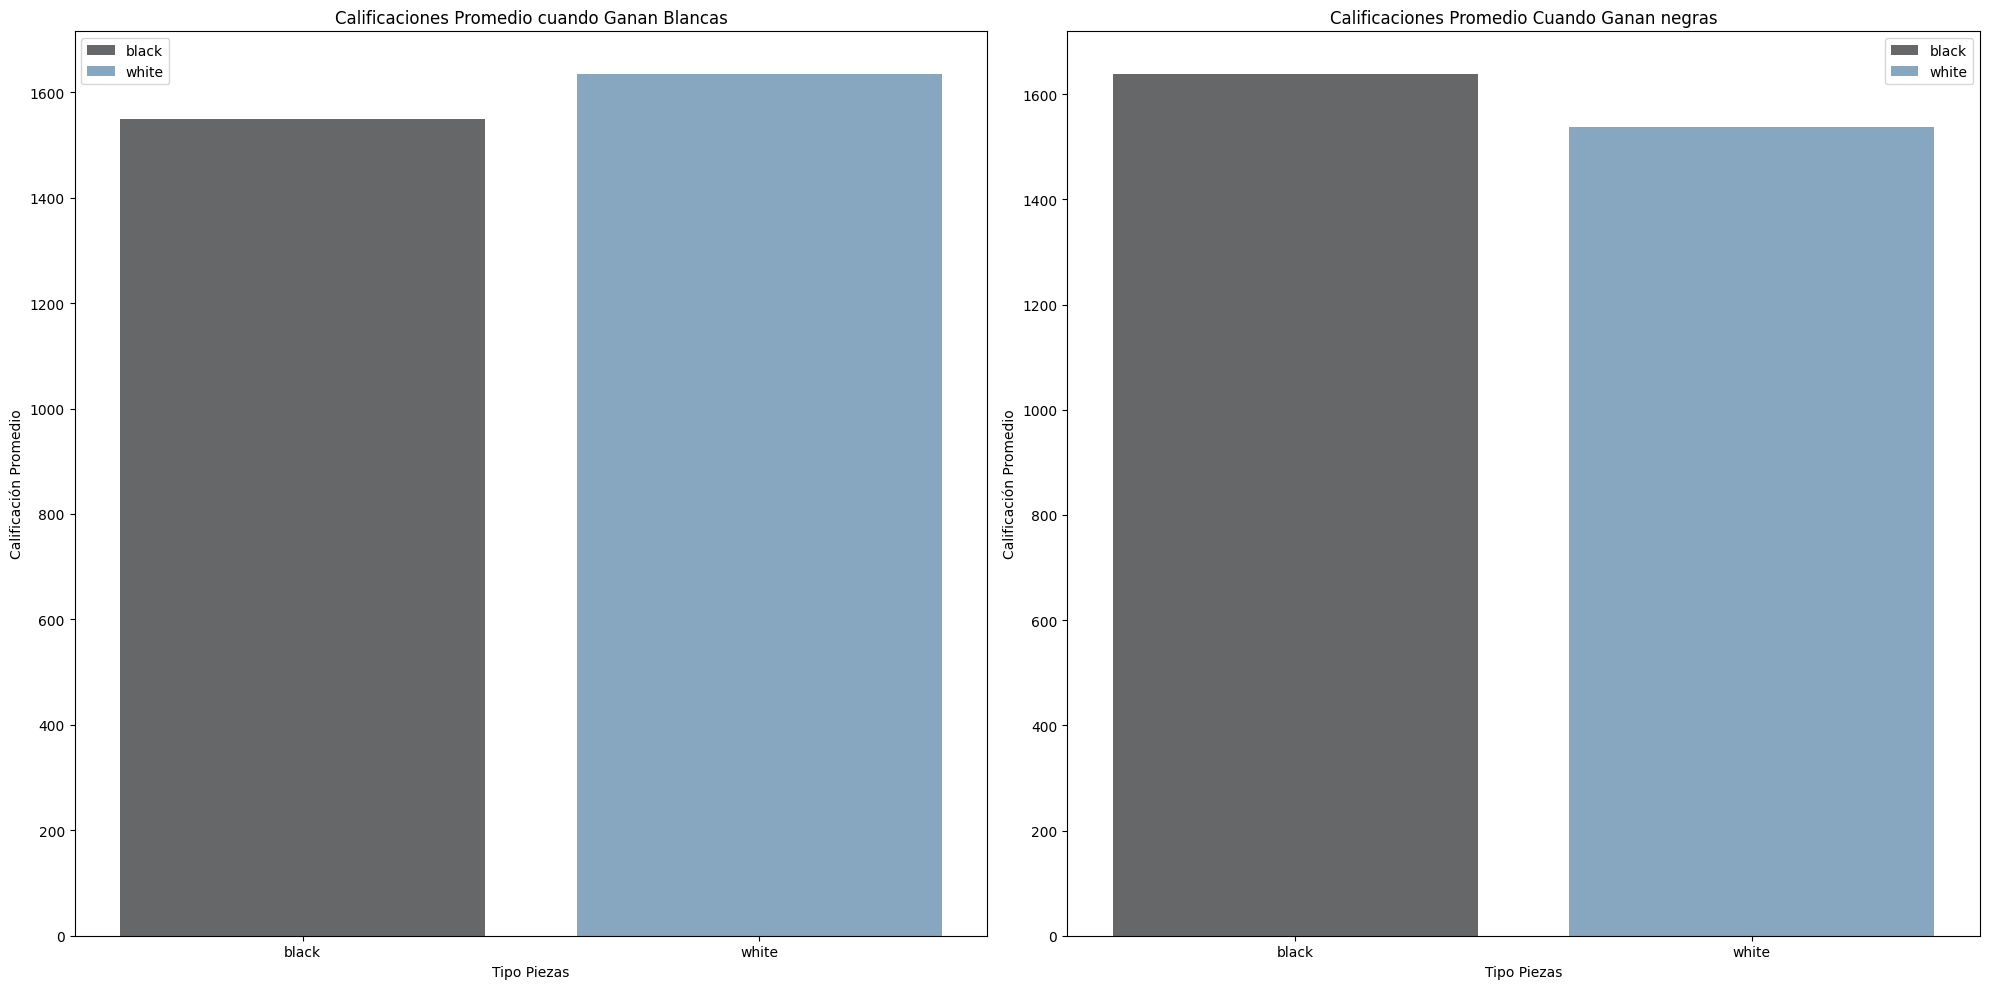
\includegraphics[width=\textwidth]{../Imagenes/Hipotesis_1.png}
    \caption{Calificaciones promedio de los ganadores y perdedores}
    \label{fig:ratings_winners_losers}
\end{figure}

%\vspace{1mm} % Espacio entre tablas

\begin{table}[h!]
    \centering
    \begin{tabular}{|c|c|}
        \hline
        \textbf{winner} & \textbf{white\_rating} \\ \hline
        black & 1549.161117 \\ \hline
        white & 1633.757659 \\ \hline
    \end{tabular}
    \caption{Tabla de ganadores cuando ganan Blancas}
    \label{table:white_rating}
\end{table}

%\vspace{1mm} % Espacio entre tablas

\begin{table}[h!]
    \centering
    \begin{tabular}{|c|c|}
        \hline
        \textbf{winner} & \textbf{black\_rating} \\ \hline
        black & 1637.666891 \\ \hline
        white & 1538.560151 \\ \hline
    \end{tabular}
    \caption{Tabla de ganadores cuando ganan Negras}
    \label{table:black_rating}
\end{table}

%\vspace{1mm} % Espacio entre tablas

\begin{table}[h!]
    \centering
    \begin{tabular}{|c|c|c|c|c|}
        \hline
        & \multicolumn{2}{|c|}{\textbf{Ganan Blancas}} & \multicolumn{2}{|c|}{\textbf{Ganan Negras}} \\ \hline
        \textbf{metdod} & \textbf{u-stat} & \textbf{p-valor} & \textbf{u-stat} & \textbf{p-valor} \\ \hline
        \textbf{t-student} & 20.23 & 4.11E-90 & 23.71 & 1.69E-122 \\ \hline
        \textbf{Mann-Whitney} & 50495725.5 & 1.92E-76 & 51737988.5 & 4.98E-106 \\ \hline
    \end{tabular}
    \caption{Comparación de métodos para ganadores con piezas blancas y negras}
    \label{table:comparison}
\end{table}

\newpage

\subsection{Hipótesis 2: El resultado de la partida depende del tipo de apertura utilizado, es decir ciertas aperturas específicas tienen una mayor tasa de victorias para las blancas o las negras}

Al comparar 2 Variables Categoricas, se realizó una prueba de chi-cuadrado para comparar las tasas de victorias entre diferentes aperturas. El test chi-2 tiene como hipótesis nula (o de partida) 
la independencia de las variables, por tanto como hemos obtenido un $p$-value $< 0{,}05$. podemos rechazar la hipótesis de partida con seguridad y pensar que existe una relación estadísticamente significativa, 
por lo que podemos decir que ciertas aperturas favorecen a un jugador sobre el otro.

\vspace{5mm} % Espacio entre tablas

Por otro lado se hizo una agrupacion por tipo de apertura y ganador para ver la distribucion y ver como se relacionaba el tipo de apertura con las victorrias tanto de piezas blancas como negras, obteniendo un mapa de calor y un $p$-value $< 0{,}05$, 
por lo que tambien podemos decir que determinadas aperturas estan relacionadas con victorias de las peizas blancas o piezas negras 


\begin{figure}[H]
    \centering
    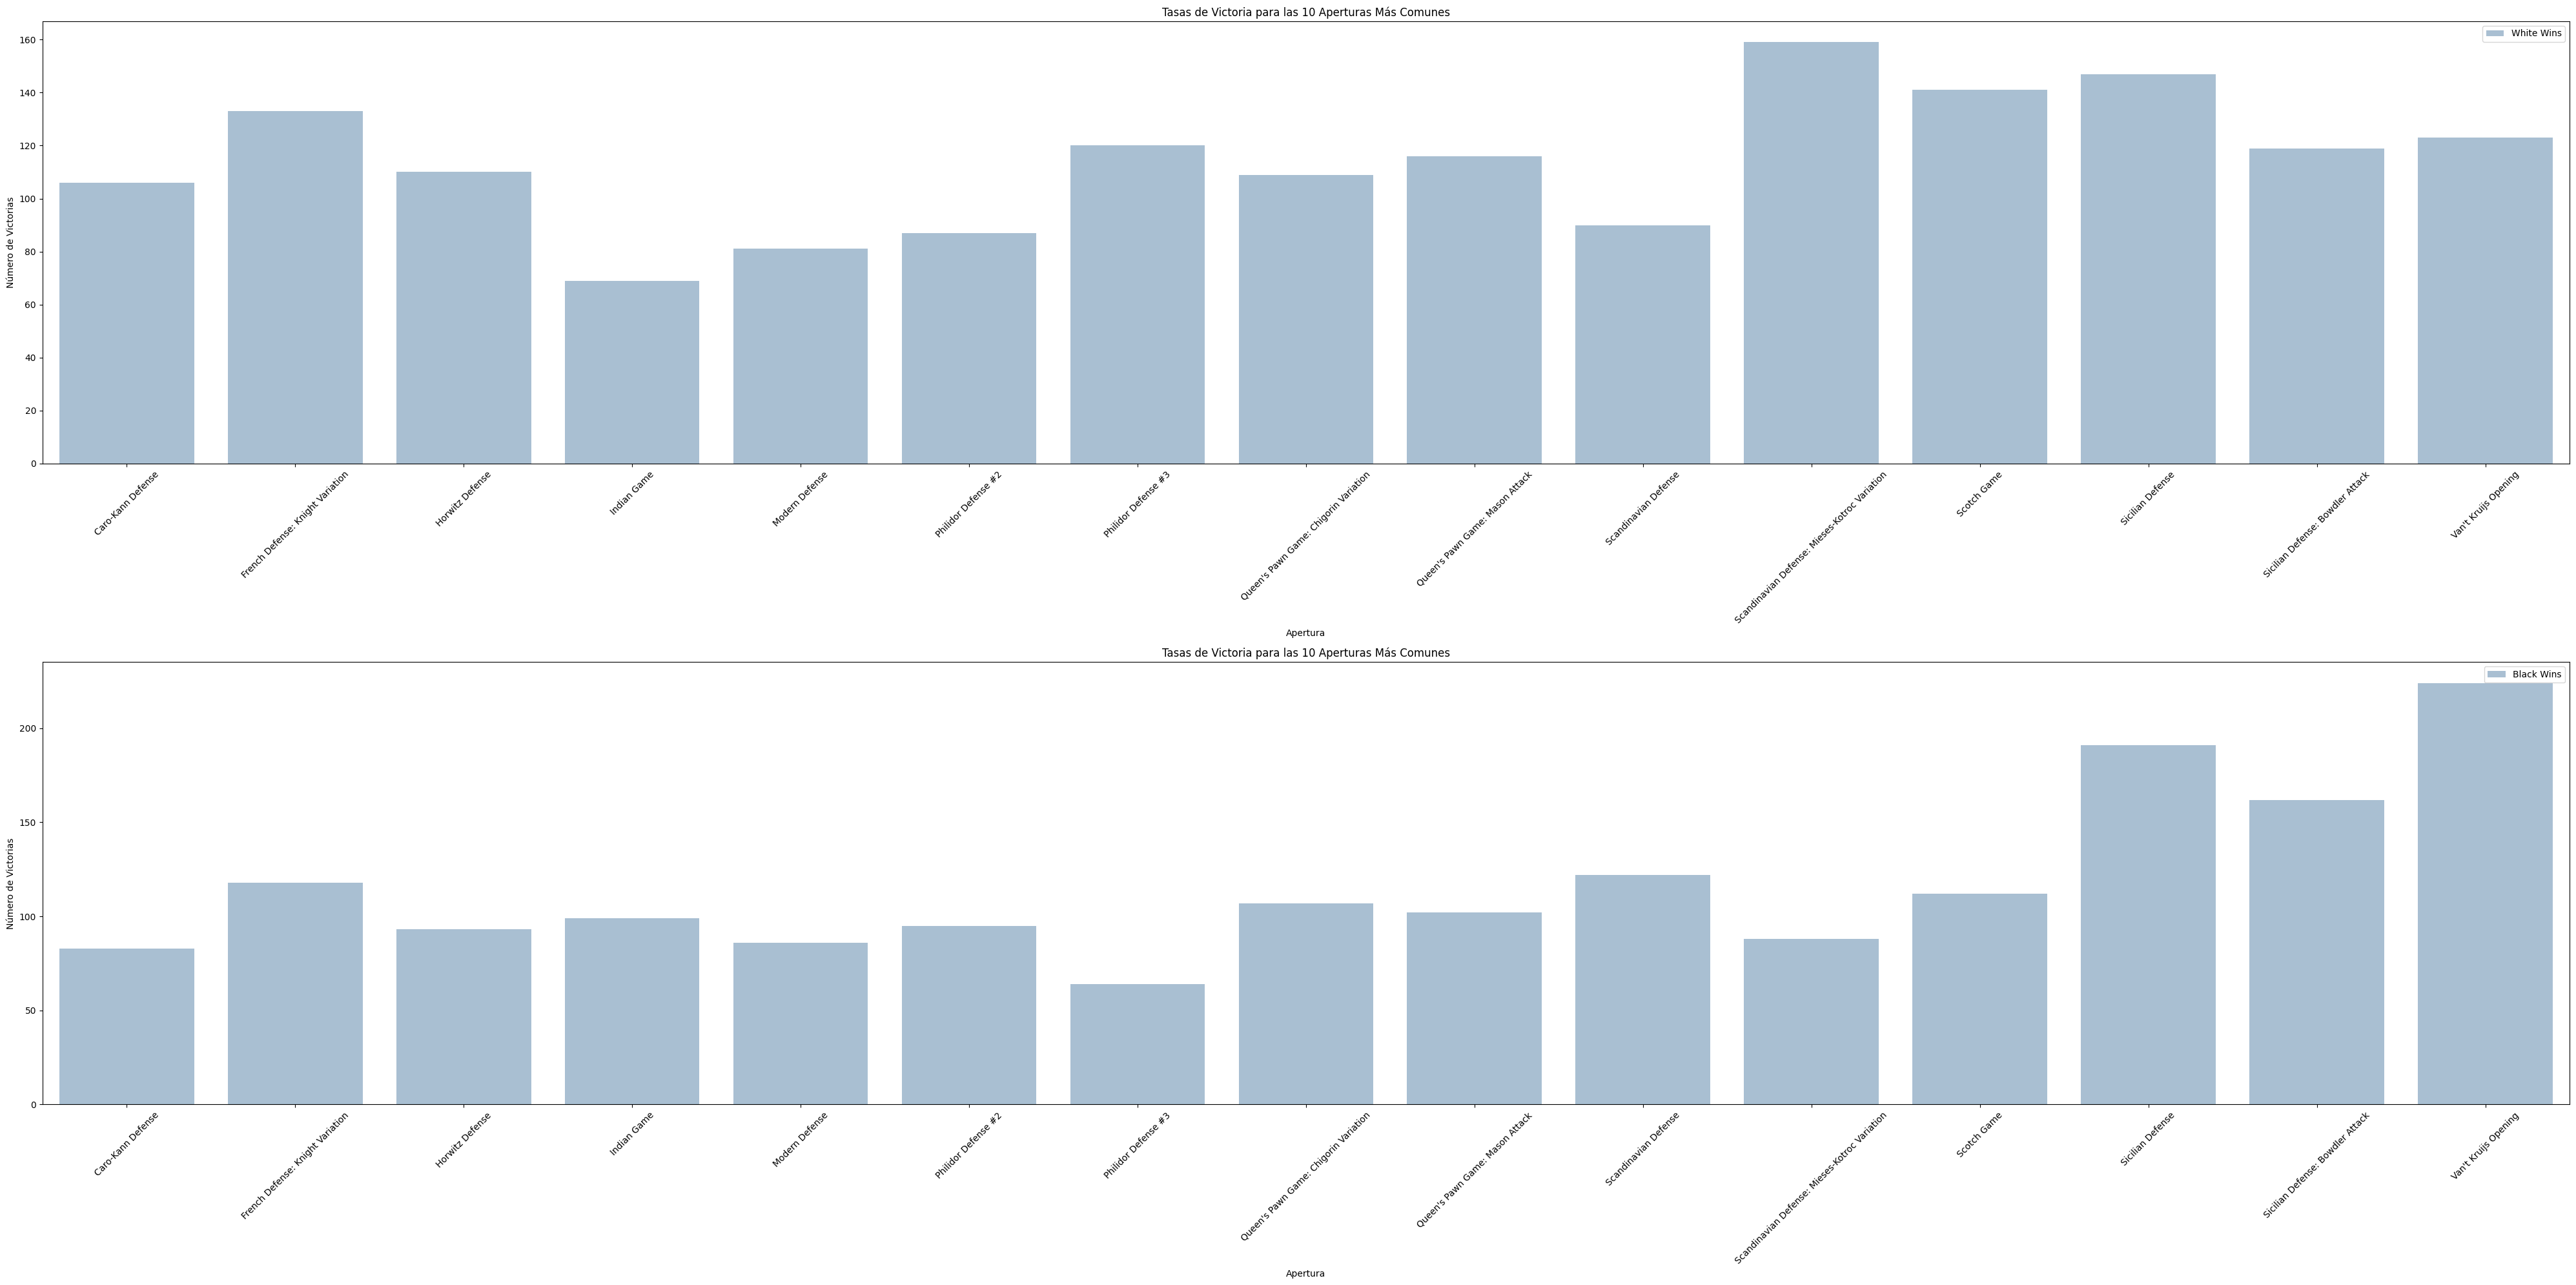
\includegraphics[width=\textwidth]{../Imagenes/Hipotesis_2.png}
    \caption{Distribución de turnos por estado de victoria}
    \label{fig:turns_victory_status}
\end{figure}

\begin{table}[h!]
    \centering
    \begin{tabular}{|c|c|}
        \hline
        \multicolumn{2}{|c|}{\textbf{Chi-Cuadrado}} \\ \hline
        \textbf{Chi-Cuadrado} & 110.15 \\ \hline
        \textbf{P-Value} & 1.07E-11 \\ \hline
        \textbf{Grados de Libertad} & 28 \\ \hline
    \end{tabular}
    \caption{Resultados del Test de Chi-Cuadrado}
    \label{table:chi_squared}
\end{table}

\begin{figure}[H]
    \centering
    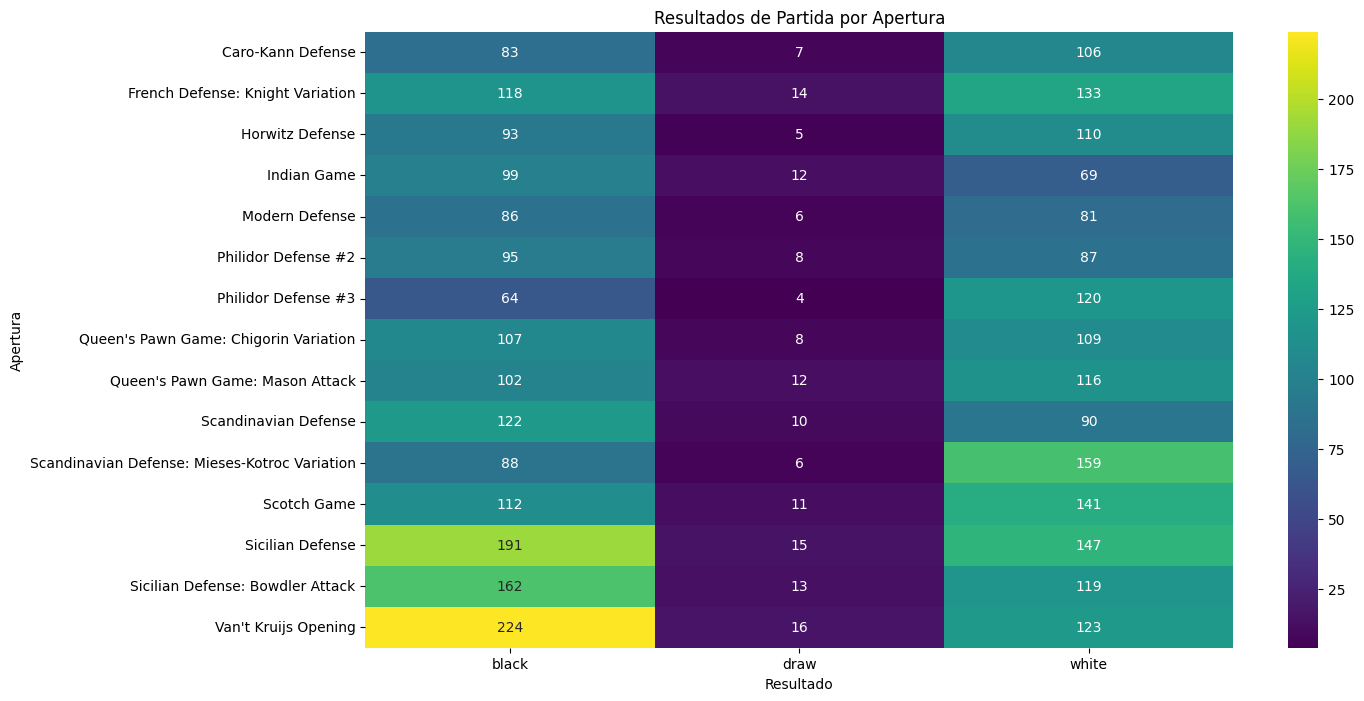
\includegraphics[width=\textwidth]{../Imagenes/Hipotesis_2_2.png}
    \caption{Resultados de partida por apertura}
    \label{fig:results_opening}
\end{figure}

\newpage

\subsection{Hipótesis 3: Las partidas con un mayor número de turnos tienden a terminar en tablas}
Se utilizó ANOVA para comparar las medias de tres o más grupos para ver si al menos uno de los grupos difiere significativamente de los demás. En este caso, estamos comparando el número de turnos entre diferentes tipos de resultados.
En este caso, el valor p es 2.3e-28, que es $p$-value $< 0{,}05$. 
Por lo tanto, rechazamos la hipótesis nula y concluimos que hay una diferencia significativa en el número de turnos entre los diferentes estados de victoria. Esto respalda la hipótesis de que las partidas con un mayor número de turnos tienden a terminar en tablas.

\begin{figure}[H]
    \centering
    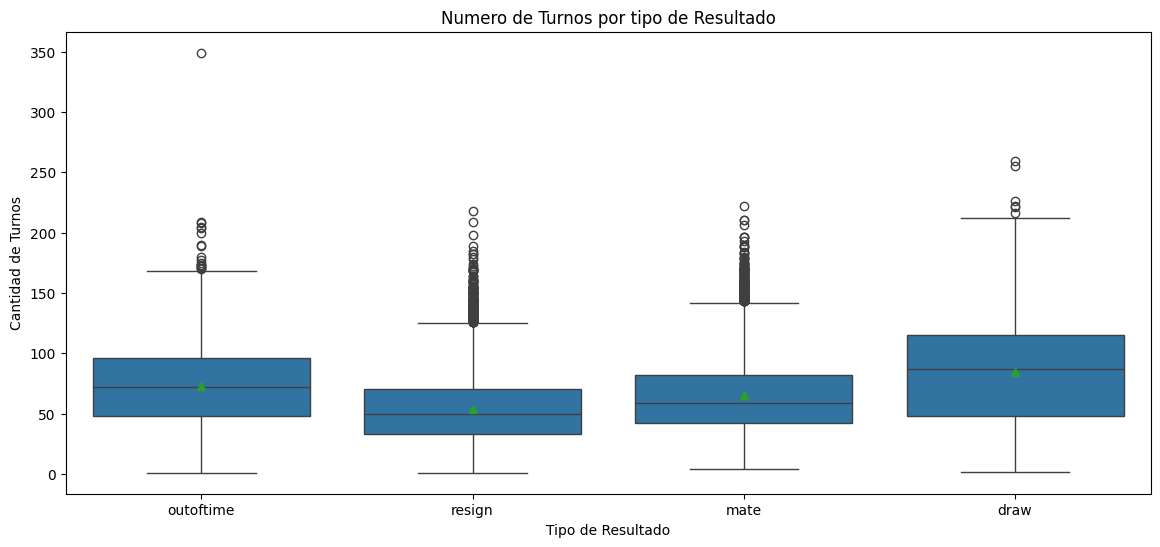
\includegraphics[width=\textwidth]{../Imagenes/Hipotesis_3.png}
    \caption{Tasas de victoria para las 10 aperturas más comunes}
    \label{fig:opening_win_rates}
\end{figure}


\begin{table}[h!]
    \centering
    \begin{tabular}{|c|c|}
        \hline
        \multicolumn{2}{|c|}{\textbf{Anova}} \\ \hline
        \textbf{f\_val} & 436.56 \\ \hline
        \textbf{p\_val} & 1.37E-274 \\ \hline
    \end{tabular}
    \caption{Resultados del Análisis de Varianza (ANOVA)}
    \label{table:anova}
\end{table}


\newpage

\section{Conclusiones}

\subsection{Hipótesis 1: Los jugadores con una calificación más alta tienden a ganar más partidas}
La calificación de los jugadores es un indicador significativo del éxito en el ajedrez. Los jugadores con calificaciones más altas tienden a ganar más partidas. Esto sugiere que la experiencia y habilidad reflejada en la calificación de un jugador es un factor crucial para el éxito en las partidas de ajedrez.

\subsection{Hipótesis 2: El resultado de la partida depende del tipo de apertura utilizado, es decir ciertas aperturas específicas tienen una mayor tasa de victorias para las blancas o las negras}
Las aperturas juegan un papel fundamental en el resultado de las partidas. Ciertas aperturas favorecen significativamente a un jugador sobre el otro, y el tipo de apertura utilizada puede determinar en gran medida si la partida será ganada por las blancas o las negras. Esto subraya la importancia de la preparación y el conocimiento de las aperturas en el ajedrez competitivo.

\subsection{Hipótesis 3: Las partidas con un mayor número de turnos tienden a terminar en tablas}
Las partidas que terminan en tablas tienden a tener un mayor número de turnos en comparación con las que terminan en jaque mate, abandono o tiempo agotado. Esto indica que las partidas más prolongadas y equilibradas, donde ninguno de los jugadores comete errores decisivos, suelen terminar en tablas. La duración de una partida puede, por lo tanto, ser un indicador de un juego bien igualado.

\subsection{Conclusión final}
El análisis de los datos revela que varios factores influyen de manera significativa en el resultado de una partida de ajedrez. La calificación del jugador, la duración de la partida y las estrategias de apertura son determinantes. Los jugadores de mayor calificación tienen una ventaja inherente, las partidas más largas tienden a ser más equilibradas, y el conocimiento y uso efectivo de las aperturas pueden cambiar el curso de una partida.

\vspace{5mm} % Espacio entre tablas
En resumen, el éxito en el ajedrez depende de una combinación de habilidad y estrategia. Los jugadores deben trabajar en mejorar su calificación a través de la práctica y el estudio, entender la importancia de la duración y el equilibrio en el juego, y dominar una variedad de aperturas para aumentar sus posibilidades de victoria.

\vspace{5mm}% Espacio entre tablas
Estas conclusiones proporcionan una visión integral de los aspectos críticos que deben ser considerados por los jugadores que buscan mejorar su rendimiento en el ajedrez.

\end{document}